\documentclass{article}
\usepackage[a4paper, total={6in, 8in}]{geometry}
\usepackage{amsmath}
\usepackage{changepage}
\usepackage{multirow}
\usepackage{tocloft}
\usepackage{tabularx}
\usepackage{graphicx}
\usepackage{array}
\usepackage{tabu}
\usepackage{longtable}
\usepackage{wrapfig}
\usepackage{verbatim}
\usepackage{xltabular}
\usepackage{listings}
\usepackage[usenames,dvipsnames,table]{xcolor}
\usepackage{pgf-umlcd}
\usepackage{pgf-umlsd}
\usepackage{tikz}
\usepackage{hyperref}
\usepackage{makecell}
\usepackage{pdfpages}
\let\cleardoublepage=\clearpage

\hypersetup{
    colorlinks=true,
    linkcolor=black,
    filecolor=magenta,
    urlcolor=cyan,
}

\lstset{
    basicstyle=\ttfamily\small,
    breaklines=true,
    frame=single,
    keywordstyle=\color{blue},
    stringstyle=\color{red},
    commentstyle=\color{green!70!black},
    showstringspaces=false,
    numbers=left,
    numberstyle=\tiny,
    numbersep=8pt,
    stepnumber=1,
    tabsize=4,
}

%creazione dei colori custom
\definecolor{tableGreen}{RGB}{25, 175, 45}
\definecolor{tableYellow}{RGB}{255, 220, 0}
\definecolor{tableBlue}{RGB}{0 ,20, 210}
\definecolor{tableCyan}{RGB}{0 ,160, 156}
\definecolor{tableRed}{RGB}{235 ,15, 0}

%macro per andare a capo nelle tabelle
\newcommand{\n}{
    \tabularnewline\hline
}

%robe per tabelle
\renewcommand{\arraystretch}{2.4}%padding sopra sotto
\setlength\tabcolsep{6pt}%padding bordo lat


%macro per generare le tabelle
\newcommand{\monkeytable}[2]{
    \begin{center}
        \begin{tabularx}{\textwidth}
            #2
            \n %necessaria per chiudere la tabella
        \end{tabularx}
    \end{center}
    \label{tab:monkeytable}
}


\newcommand{\subsubsubsection}[1]{\paragraph{#1}\mbox{}\\}
% Modifica del contatore di profondità
\setcounter{secnumdepth}{4}
\setcounter{tocdepth}{4}


\pagestyle{fancy}
\fancyhf{} % Rimuove l'header e il footer predefiniti
\renewcommand{\headrulewidth}{0pt} % Rimuove la linea dell'header
\rfoot{} % Imposta solo il numero di pagina nel footer destro

\title{Codemonkey}
\begin{document}

\begin{figure}[!ht]
   \centering
   % 
\includegraphics[width=0.5\linewidth]{assets/img/icon}
   \begin{titlepage}
      \huge Codemonkey
   \end{titlepage}\label{fig:nome-etichetta}
\end{figure}

\renewcommand{\contentsname}{Sommario}
\tableofcontents

\pagebreak

%%%%%%%%%%%%%%%%%%%%

\subsection{Abstract}
\subsection {Abstract}

L'obiettivo è sviluppare una piattaforma web che espone programmatori a realtà lavorative che ne hanno bisogno.
Sia i programmatori che le aziende si registrano al sito, e sono interfacciati al servizio Codemonkey attraverso pannelli diversi.
Un programmatore registrato inserisce i propri contatti, una breve descrizione e un elenco degli strumenti software nei quali ha competenze.
Un'azienda registrata può cercare programmatori filtrandoli per gli strumenti software dei quali ha esigenza. Quando l'azienda sceglie un programmatore, a questo arriva una notifica e può decidere di accettare il lavoro.
A lavoro concluso, l'azienda valuta il programmatore con un sistema di quotazione.
Il profilo del programmatore è aggiornato con i suoi lavori recenti.

\pagebreak

%%%%%%%%%%%%%%%%%%%%

\section{Analisi dei requisiti}
\subsection{Raccolta dei requisiti}
\begin{itemize}
\large
\item Gli utenti del servizio Codemonkey si registrano da una pagina e indicano se intendono registrarsi come Codemonkey o Clienti
\item La Codemonkey potrá accedere, modificare i suoi dati e accettare eventuali lavori dopo aver eseguito l'Autenticazione
\item Un Cliente potrá accedere, modificare i suoi dati e gestire le Collaborazioni dopo aver eseguito il l'Autenticazione
\item Gli Utenti possono sfogliare il sito. Solo i clienti possono mandare richieste di Lavoro alle Codemonkey
\item Le Codemonkey possono accettare o rifiutare i lavori
\item I clienti possono valutare la Codemonkey solo dopo aver terminato la collaborazione e la valutazione potrá ache opzionalmente contenere una recensione
\item Si potranno cercare Codemonkey utlizzando dei filtri specifici
\end{itemize}

\subsection{Vocabolario}
\begin{center}

    \rowcolors{2}{orange!20}{orange!5}%colori alternati

    \resizebox{1\textwidth}{!}{
        \begin{tabular}
            {|>{\raggedright}m{3cm}|>{\raggedright}m{9cm}|m{3cm}|}%Opzioni per formato tabella
            \hline %riga in cima alla colonna    
            \rowcolor{orange!50}%settare il colore della colonna principale 
            \Large\textbf{Voce}    & \Large\centering\textbf{Definizione}                                                                              & \Large\textbf{Sinonimo} %voci della prima colonna
            \n  Utente             & Persona non autenticata che usufruisce della piattaforma                                                          &
            \n  Nome Utente        & Stringa alfanumerica che identifica il nome di un Utente                                                          & Username
            \n  Chiave di accesso  & Stringa alfanumerica scelta da un utente, da tenere segreta                                                       & Password
            \n  TOTP               & Time-based One-Time Password, codice numerico generato dal sistema, utilizzato per l'autenticazione a due fattori &
            \n  Registrazione      & Funzione di iscrizione alla piattaforma                                                                           &
            \n  Autenticazione     & Metodo di accesso al servizio, basato su Username, Password e TOTP                                                & Log in
            \n  Utente autenticato & Utente che ha effettuato l'autenticazione                                                                         &
            \n  Amministratore     & Addetto alla manutenzione della piattaforma                                                                       & Admin
            \n  Codemonkey         & Utente registrato o autenticato come programmatore                                                                &
            \n  Cliente            & Azienda o un semplice privato interessato a utilizzare servizi offerti dalle Codemonkey                           &
            \n  Profilo Completo   & Il profilo di una Codemonkey è completo se sono presenti tutte le informazioni richieste dalla piattaforma        &
            \n
        \end{tabular}\label{tab:monkeytable:vocabolario1}}

    \resizebox{1\textwidth}{!}{
        \begin{tabular}
            {|>{\raggedright}m{3cm}|>{\raggedright}m{9cm}|m{3cm}|}%Opzioni per formato tabella
            \hline %riga in cima alla colonna    
            \rowcolor{orange!50}%settare il colore della colonna principale 
            \Large\textbf{Voce}                 & \Large\centering\textbf{Definizione}                                                                                                                                                                                                                                                             & \Large\textbf{Sinonimo}          %voci della prima colonna
            \n  Collaborazione                          & Contratto tra una Codemonkey e un Cliente per lo sviluppo di un progetto software. Può essere \textit{proposto} da un Cliente ed \textit{accettato} o \textit{rifiutato} da una Codemonkey. Se viene accettato, può essere \textit{interrotto} dalla Codemonkey o \textit{terminato} dal Cliente & Progetto,\newline Lavoro
            \n  Tag                             & Parole chiave che permettono di trovare le Codemonkey, saranno quindi i linguaggi di programmazione e le applicazioni che sono in grado di utilizzare                                                                                                                                            & Filtro
            \n  Ricerca                         & Il modo in cui si possono trovare le Codemonkey, si basa sui Tag                                                                                                                                                                                                                                 & Feed
            \n  Valutazione                     & Valore espresso in stelle da 1 a 5 per quantificare le prestazioni di una Codemonkey                                                                                                                                                                                                             &
            \n  Valutazione Filtrata            & Valutazione media di una Codemonkey in base ai Tag impostati                                                                                                                                                                                                                                     &
            \n  Recensione                      & Commento scritto da un Cliente per valutare le prestazioni di una Codemonkey                                                                                                                                                                                                                     &
            \n Segnalazione                    & Messaggio inviato da un Utente per segnalare un comportamento scorretto                                                                                                                                                                                                                          & Report
            
            \n  (Cliente) Limitato              & Cliente che non ha diritto di lasciare Recensioni                                                                                                                                                                                                                                                &
            \n  (Cliente o Codemonkey) Sospeso  & Utente che non ha diritto di avviare o accettare Lavori                                                                                                                                                                                                                                          &
            \n  (Cliente o Codemonkey) Bloccato & Utente che non ha diritto di accedere alla piattaforma                                                                                                                                                                                                                                           & Ban
            \n
        \end{tabular}\label{tab:monkeytable:vocabolario2}}
\end{center}


\subsection{Tabelle requisiti}
\subsubsection{Requisiti funzionali}
\newcounter{reqFCounter}%counter

\newcommand{\nReqF}{
    \n
    \stepcounter{reqFCounter}
    R\thereqFCounter F
}

\begin{center}
    \rowcolors{2}{tableGreen!5}{tableGreen!15}%colori alternati
    
    \begin{tabularx}{\textwidth}
        {|c|X|}
        \hline\rowcolor{tableGreen!70}
        \multicolumn{2}{|c|}{\Large\textbf{Requisiti Funzionali}}
        \n \rowcolor{tableGreen!50}

        \large\textbf{ID}
               & \large\textbf{Requisito}
        \nReqF & Deve esistere un sistema per Registrare nuovi Utenti
        \nReqF & Deve essere disposto un sistema di Autenticazione per Utenti giá Registrati
        \nReqF & Deve essere possibile eseguire una Ricerca di Codemonkey con utilizzo di Filtri                                                                       % insomma da rivedere ammodo (valerio scassapalle)
        \nReqF & Una Codemonkey e un Cliente potranno modificare l'e-mail e la Password legate all'Account
        \nReqF & Una Codemonkey e un Cliente potranno modificare la propria descrizione, nome Utente, immagine di profilo e contatti associati all'account
        \nReqF & Una Codemonkey e un Cliente potranno visualizzare tutte le richieste di Lavoro che li riguardano
        \nReqF & Una Codemonkey e un Cliente possono in qualsiasi momento effettuare una segnalazione su una Collaborazione % o un profilo
        \nReqF & Una Codemonkey deve poter gestire i propri Tag di Ricerca
        \nReqF & Una Codemonkey dovrá avere la possibilitá di Accettare o Rifiutare una proposta di Lavoro presentata da un Cliente
        \nReqF & Una Codemonkey avrá la possibilitá di Interrompere una Collaborazione con un Cliente
        \nReqF & Una Codemonkey potrá essere visualizzata solo se ha un Profilo Completo                                                                               % da spostare reqD
        \nReqF & Un Cliente puó effettuare proposte di lavoro ad una Codemonkey
        \nReqF & Un Cliente potrá terminare una Collaborazione con una Codemonkey fornendo una valutazione e potrá inoltre scrivere una breve recensione
        \n
    \end{tabularx}

    \begin{tabularx}{\textwidth}
        {|c|X|}
        \hline\rowcolor{tableGreen!70}
        \multicolumn{2}{|c|}{\Large\textbf{Requisiti Funzionali}}
        \n \rowcolor{tableGreen!50}

        \large\textbf{ID}
               & \large\textbf{Requisito}
        \nReqF & Un Amministratore deve poter essere in grado di Eliminare, Bloccare, Sospendere e Limitare qualsiasi Utente Registrato
        \nReqF & Un Amministratore deve approvare i Tag non pre esistenti inseriti dalle Codemonkey
        \nReqF & Un Amministratore deve poter visualizzare le segnalazioni effettuate dagli Utenti Registrati
        \nReqF & Un Cliente in stato di sospensione non potrá piú contattare nuove Codemonkey, potrá solo portare a termine i Lavori giá avviati
        \nReqF & Una Codemonkey sospesa non deve piú comparire nelle ricerche effettuate dagli Utenti
        \nReqF & Un Utente Registrato quando viene Bloccato termina immediatamente tutte le collaborazioni e non potrá piú avviarne di nuove
        \n
    \end{tabularx}
\end{center}
\subsubsection{Requisiti non funzionali}
\newcounter{reqNFCounter} %counter

\newcommand{\nReqNF}{
    \n
    \stepcounter{reqNFCounter}
    R\thereqNFCounter NF
}

\begin{center}
    \rowcolors{2}{tableYellow!5}{tableYellow!10} %colori alternati
    \begin{tabularx}{\textwidth}
        {|c|X|}
        \hline \rowcolor{tableYellow!55}
        \large\textbf{ID}
                & \large\textbf{Requisito}
        \nReqNF & Il sito deve essere facile da navigare
        \nReqNF & Sará possibile vedere a quali Collaborazioni la Codemonkey ha preso parte
        \nReqNF & Il sito avrà facilitazioni per l'accessibilità, compresa una modalità "Scura"
        \nReqNF  & Una Codemonkey sospesa non deve piú comparire nelle ricerche effettuate dagli Utenti
        \n
    \end{tabularx}
\end{center}
\subsubsection{Requisiti di dominio}
\newcounter{reqDCounter}%counter

\newcommand{\nReqD}{
    \n
    \stepcounter{reqDCounter}
    R\thereqDCounter D
}

\begin{center}
    \rowcolors{2}{tableBlue!4}{tableBlue!8}%colori alternati
    \begin{tabularx}{\textwidth}
        {|c|X|}
        \hline\rowcolor{tableBlue!50}
        \multicolumn{2}{|c|}{\Large\textbf{Requisiti di Dominio}}
        \n \rowcolor{tableBlue!25} \large\textbf{ID}
               & \large\textbf{Requisito}
        \nReqD & Non é necessaria l'autenticazione per eseguire una Ricerca di Codemonkey
        \nReqD & Gli Amministratori del sistema devono essere creati prima dell'avvio del sistema e non se ne possono aggiungere altri durante l'esecuzione
        \nReqD & Non sará possibile regisrtarsi sia come Codemonkey che come Cliente
        \nReqD & Un Utente Registrato in qualsiasi momento puó richiedere l'eliminazione del suo Account
        \n
    \end{tabularx}
\end{center}

\subsection{Scenari}
\newcommand{\tableCyan}{%righe con colori misti inseriti dentro
    \n
    \rowcolor{tableCyan!10}
    \cellcolor{tableCyan!22}
}

\newcommand{\ntableCyan}{%righe con colori misti inseriti dentro
    \n
    \rowcolor{tableCyan!5}
    \cellcolor{tableCyan!12}
}

%%%%%%%%%%%%%%%%%%%%%%%%%%%

\begin{tabularx}{\textwidth}
    {|>{\arraybackslash}m{3cm}|>{\arraybackslash}X|}

    \hline  \rowcolor{tableCyan!37}
    \large\centering\textbf{Titolo}     & \large\centering\textbf{Homepage}
    \tableCyan      Descrizione         & Sezione principale nella quale si possono eseguire ricerche di Codemonkey
    \ntableCyan     Attori              & Utente, Cliente
    \tableCyan      Relazioni           &
    \ntableCyan     Precondizioni       &
    \tableCyan      Postcondizioni      &
    \ntableCyan     Scenario Principale & Un Utente attraverso l'utilizzo di Tag puó trovare la Codemonkey ideale per sviluppare il suo progetto
    \tableCyan      Scenari Alternativi &
    \ntableCyan     Requisiti NF        & Interfaccia grafica intuitiva e dall'estetica pulita
	\tableCyan      Punti Aperti        & Per efficienza nell'esecuzione del sistema, non si potranno scaricare tutti i profili aderenti ai Tag in una sola volta, come si potrebbe implementare? Si potrà scaricare la lista delle Codemonkey aderenti ai Tag in? Come funzionerà il caricamento di nuovi profili un avolta raggiunta la fine della pagina?
    \n
\end{tabularx}

%%%%%%%%%%%%%%%%%%%%%%%%%%%%

\begin{tabularx}{\textwidth}
    {|m{3cm}|X|}
    \hline \rowcolor{tableCyan!40}
    \large\centering\textbf{Titolo}     & \large \centering\textbf{Registrazione}
    \tableCyan      Descrizione         & Sezione che consente la Registrazione di un Utente
    \ntableCyan     Attori              & Utente
    \tableCyan      Relazioni           &
    \ntableCyan     Precondizioni       &
    \tableCyan      Postcondizioni      & L'Utente viene registrato nel sistema come Codemonkey o come Cliente
    \ntableCyan     Scenario Principale &
    \begin{enumerate}
        \item L'Utente inserisce le credenziali (Username, Email, Password) per la creazione di un Account
        \item L'Utente specifica se vuole essere registrato come Cliente o Codemonkey
        \item L'Utente conferma di volersi registrare
    \end{enumerate}
    \tableCyan      Scenari Alternativi & Se lo Username é giá stato scelto o l'Email immessa é collegata a un Account giá registrato non sará possibile procedere alla Registrazione dell'Utente
    \ntableCyan     Requisiti NF        & Sia nel caso in cui venga inserito un Username giá esistente, sia nel caso venga inserita una Email associata ad un Account esistente, dovrá essere segnalato all'Utente che non é stato possibile effettuare la Registrazione spiegandone la motivazione
    \tableCyan      Punti Aperti        & Verrá abilitata l'autenticazione a 2 fattori giá in fase di Registrazione?\newline
    Bisognerá assicurarsi che l'Utente non si sbagli a digitare la Password, ci sarà un campo di conferma Password?
    \n
\end{tabularx}
\begin{tabularx}{\textwidth}
    {|>{\arraybackslash}m{3cm}|>{\arraybackslash}X|}

    \hline \rowcolor{tableCyan!37}
    \large\centering\textbf{Titolo}     & \large\centering\textbf{Autenticazione}
    \tableCyan      Descrizione         & Sezione dedicata all'Autenticazione di un Utente
    \ntableCyan     Attori              & Utente
    \tableCyan      Relazioni           & Gestione Profilo, Proponi Lavoro, Fornisci recensione, Area personale, Gestione Utenti  
    \ntableCyan     Precondizioni       & L'Utente deve essere giá registrato all'interno del sistema oppure deve essere un Amministratore.
    \tableCyan      Postcondizioni      & L'Utente sarà Utente Autenticato oppure Amministratore.
    \ntableCyan     Scenario Principale &
    \begin{enumerate}
        \item L'Utente fornisce le credenziali di accesso al sistema
        \item L'Utente conferma di voler entrare con le credenziali immesse
        \item Nel caso in cui le credenziali siano corrette, Codemonkey o Cliente saranno reindirizzati alla Gestione del Profilo, invece l'Amministratore sará reindirizzato verso la Gestione del Sistema
    \end{enumerate}
    \tableCyan      Scenari Alternativi & Nel caso che i dati forniti per l'autenticazione siano incorretti verrá visualizzato un messaggio di errore\newline Nel caso l'utente sia stato bloccato da un Amministratore verrá fornito un messaggio di errore.
    \ntableCyan     Requisiti NF        & Sará sempre presente un bottone per inoltrare una richiesta di recupero Password all'Amministratore.
    \tableCyan      Punti Aperti        & 
    \n
\end{tabularx}

%%%%%%%%%%%%%%%%%%%%%%%%%%%%

\begin{tabularx}{\textwidth}
    {|>{\arraybackslash}m{3cm}|>{\arraybackslash}X|}

    \hline \rowcolor{tableCyan!37}
    \large\centering\textbf{Titolo}     & \large\centering\textbf{Gestione Profilo}
    \tableCyan      Descrizione         & Sezione dedicata alla gestione dei dati di un Account
    \ntableCyan     Attori              & Cliente, Codemonkey
    \tableCyan      Relazioni           & Autenticazione
    \ntableCyan     Precondizioni       & La Codemonkey o il Cliente devono aver effettuato l'Autenticazione
    \tableCyan      Postcondizioni      &
    \ntableCyan     Scenario Principale &
    \begin{enumerate}
        \item Un Utente Autenticato accede alla funzionalitá di Gestione Account
        \item L'Utente Autenticato potrá quindi modificare Password, Email
        \item Le modifiche apportate quindi saranno salvate solo se confermate dall'utente
    \end{enumerate}
    \tableCyan      Scenari Alternativi & 2.1. Una Codemonkey potrà modificare i propri Tag
    \ntableCyan     Requisiti NF        &
    \tableCyan      Punti Aperti        & Se un Utente Registrato cambia la sua email potrebbero esserci incomprensioni?
    \n
\end{tabularx}

%%%%%%%%%%%%%%%%%%%%%%%%%%%%

\begin{tabularx}{\textwidth}
    {|>{\arraybackslash}m{3cm}|>{\arraybackslash}X|}

    \hline \rowcolor{tableCyan!37}
    \large\centering\textbf{Titolo}     & \large\centering\textbf{Imposta Tag di Ricerca}
    \tableCyan      Descrizione         & Gestione dei Tag della Codemonkey
    \ntableCyan     Attori              & Codemonkey
    \tableCyan      Relazioni           & Autenticazione
    \ntableCyan     Precondizioni       &
    \tableCyan      Postcondizioni      & I Tag vengono aggiornati
    \ntableCyan     Scenario Principale &
    \begin{enumerate}
        \item La Codemonkey apre la pagina dedicata alla gestione dei Tag
        \item La Codemonkey aggiunge o rimuove un Tag tra quelli disponibili
        \item La Codemonkey conferma i cambiamenti
    \end{enumerate}
    \tableCyan      Scenari Alternativi &
        2.1. Se il Tag che si vuole aggiungere non é presente tra quelli disponibili, la Codemonkey puó inviare una richiesta per aggiungerlo
    \ntableCyan     Requisiti NF        & I Tag vengono aggiunti digitando in una casella di testo
    \tableCyan      Punti Aperti        & Cosa succede se si tenta di aggiunere un nuovo Tag? Bisognerá che un Amministratore controlli il Tag prima di aggiungerlo?
    \n
\end{tabularx}

%%%%%%%%%%%%%%%%%%%%%%%%%%%%

\begin{tabularx}{\textwidth}
    {|>{\arraybackslash}m{3cm}|>{\arraybackslash}X|}

    \hline \rowcolor{tableCyan!37}
    \large\centering\textbf{Titolo}     & \large\centering\textbf{Segnalazione ad Amministratore}
    \tableCyan      Descrizione         & Funzionalitá per effettuare una Segnalazione ad un Amministratore
    \ntableCyan     Attori              & Codemonkey, Cliente
    \tableCyan      Relazioni           & Lista Collaborazioni
    \ntableCyan     Precondizioni       & Codemonkey e Cliente devono essere autenticati
    \tableCyan      Postcondizioni      & La richiesta sará inoltrata ad un Amministratore
    \ntableCyan     Scenario Principale &
    \begin{enumerate}
        \item La Codemonkey o il Cliente potranno avviare una Segnalazione ad un altro Utente
        \item La Codemonkey o il Cliente compilano un form per motivare la Segnalazione
        \item Viene confermata l'invio della Segnalazione
    \end{enumerate}
    \tableCyan      Scenari Alternativi &
    \ntableCyan     Requisiti NF        &
    \tableCyan      Punti Aperti        &
    \n
\end{tabularx}

%%%%%%%%%%%%%%%%%%%%%%%%%%%%

\begin{tabularx}{\textwidth}
    {|>{\arraybackslash}m{3cm}|>{\arraybackslash}X|}

    \hline  \rowcolor{tableCyan!37}
    \large\centering\textbf{Titolo}     & \large\centering\textbf{Proponi Lavoro}
    \tableCyan      Descrizione         & Sezione dedicata all'invio di una proposta di Lavoro ad una Codemonkey
    \ntableCyan     Attori              & Cliente, Utente
    \tableCyan      Relazioni           & Autenticazione
    \ntableCyan     Precondizioni       &
    \tableCyan      Postcondizioni      & La richiesta di Lavoro viene inoltrata alla Codemonkey
    \ntableCyan     Scenario Principale &
    \begin{enumerate}
        \item Un Utente o un Cliente ha trovato la Codemonkey ideale per sviluppare il suo progetto e puó proporle un Lavoro
        \item L'Utente viene reindirizzato alla sezione di Autenticazione prima di poter iniziare l'inoltro della richiesta
        \item Per mandare la richiesta di Lavoro il Cliente compila un modulo nel quale descrive brevemente l'attività che la Codemonkey svolgerà e i Tag associati a tale attività
        \item Il Cliente conferma di voler contattare la Codemonkey
    \end{enumerate}
    \tableCyan      Scenari Alternativi & 
        2.1 Un Cliente può procedere senza dovere effettuare l'Autenticazione nuovamente. 
        \newline 
        2.2 Un Cliente Sospeso non puó fare alcuna richiesta di Lavoro
    \ntableCyan     Requisiti NF        & Se il Cliente è Sospeso verrá visualizzata una pagina di errore che lo avvisa di non poter effettuare la richiesta di Lavoro
    \tableCyan      Punti Aperti        & Per evitare che vengano inviate richieste di Lavoro non sufficentemente dettagliate ci sarà un numero minimo di caratteri da inserire nel campo di testo
    \n
\end{tabularx}

%%%%%%%%%%%%%%%%%%%%%%%%%%%%

\begin{tabularx}{\textwidth}
    {|>{\arraybackslash}m{3cm}|>{\arraybackslash}X|}

    \hline \rowcolor{tableCyan!37}
    \large\centering\textbf{Titolo}     & \large\centering\textbf{Lista Collaborazioni}
    \tableCyan      Descrizione         & Lista di tutte le collaborazioni
    \ntableCyan     Attori              & Codemonkey, Cliente
    \tableCyan      Relazioni           & Gestione Profilo
    \ntableCyan     Precondizioni       & Codemonkey e Cliente devono essere autenticati
    \tableCyan      Postcondizioni      &
    \ntableCyan     Scenario Principale &
    \begin{enumerate}
        \item La Codemonkey o il Cliente dalla Gestione dell'Account potranno accedere alla Lista collaborazioni
        \item Possono visualizzare le collaborazioni attive e passate
    \end{enumerate}
    \tableCyan      Scenari Alternativi &
    \ntableCyan     Requisiti NF        & 
    \tableCyan      Punti Aperti        & Cosa succede se una Codemonkey Interrompe un Lavoro giá iniziato? Il Cliente potrà ancora effettuare una Valutazione?
    \n
\end{tabularx}

%%%%%%%%%%%%%%%%%%%%%%%%%%%%

\begin{tabularx}{\textwidth}
    {|>{\arraybackslash}m{3cm}|>{\arraybackslash}X|}

    \hline  \rowcolor{tableCyan!37}
    \large\centering\textbf{Titolo}     & \large\centering\textbf{Accetta/Rifiuta proposta di Lavoro}
    \tableCyan      Descrizione         & Sezione per la gestione delle Collaborazioni della Codemonkey
    \ntableCyan     Attori              & Codemonkey
    \tableCyan      Relazioni           & Autenticazione
    \ntableCyan     Precondizioni       & Il Lavoro é stato proposto alla Codemonkey
    \tableCyan      Postcondizioni      & Il Lavoro diventa ``in Corso''
    \ntableCyan     Scenario Principale &
    \begin{enumerate}
        \item Alla Codemonkey viene effettuata una proposta di Lavoro da parte di un Cliente
        \item La Codemonkey accetta la proposta
        \item La Codemonkey poi potrá interrompere la richiesta di Lavoro in qualsiasi momento fino a quando non viene terminata da un Cliente
    \end{enumerate}
    \tableCyan      Scenari Alternativi & 2. La Codemonkey rifiuta la proposta
    \ntableCyan     Requisiti NF        &
    \tableCyan      Punti Aperti        &
    \n
\end{tabularx}

%%%%%%%%%%%%%%%%%%%%%%%%%%%%

\begin{tabularx}{\textwidth}
    {|>{\arraybackslash}m{3cm}|>{\arraybackslash}X|}

    \hline  \rowcolor{tableCyan!37}
    \large\centering\textbf{Titolo}     & \large\centering\textbf{Interrompi Lavoro}
    \tableCyan      Descrizione         & Funzionalità per l'interruzione di una Collaborazione in corso da parte della Codemonkey
    \ntableCyan     Attori              & Codemonkey
    \tableCyan      Relazioni           & Autenticazione
    \ntableCyan     Precondizioni       & Il Lavoro é stato già accetato dalla Codemonkey
    \tableCyan      Postcondizioni      & Il Lavoro diventa ``Interrotto''
    \ntableCyan     Scenario Principale &
    \begin{enumerate}
        \item La Codemonkey sceglie un Lavoro che ha in corso per interromperlo
        \item La Codemonkey interrompe il Lavoro e aggiunge un commento sull'interruzione
    \end{enumerate}
    \tableCyan      Scenari Alternativi &
    \ntableCyan     Requisiti NF        & 
    \tableCyan      Punti Aperti        & 
    \n
\end{tabularx}


%%%%%%%%%%%%%%%%%%%%%%%%%%%%

\begin{tabularx}{\textwidth}
    {|>{\arraybackslash}m{3cm}|>{\arraybackslash}X|}

    \hline  \rowcolor{tableCyan!37}
    \large\centering\textbf{Titolo}     & \large\centering\textbf{Termina Collaborazione e Valuta Codemonkey}
    \tableCyan Descrizione              & Sezione per terminare un Lavoro e fornire una Valutazione ad una Codemonkey
    \ntableCyan     Attori              & Cliente
    \tableCyan      Relazioni           & Autenticazione
    \ntableCyan     Precondizioni       &
    \tableCyan      Postcondizioni      & Viene terminato il Lavoro
    \ntableCyan     Scenario Principale &
    \begin{enumerate}
        \item Un Cliente consulta le sue Collaborazioni attive
        \item Il Cliente avvia la procedura per terminare la Collaborazione
        \item Il Cliente Fornisce una valutazione da 0 a 5 alla Codemonkey
        \item Il Cliente puó scrivere quindi una recensione alla Codemonkey (opzionale)
        \item Il Cliente da conferma di voler terminare il Lavoro

    \end{enumerate}
    \tableCyan      Scenari Alternativi & Nel caso il Cliente sia stato Limitato o Sospeso non potrá fornire una valutazione scritta alla Codemonkey
    \ntableCyan     Requisiti NF        &
    \tableCyan      Punti Aperti        & 
    \n
\end{tabularx}


%%%%%%%%%%%%%%%%%%%%%%%%%%%%

\begin{tabularx}{\textwidth}
    {|>{\arraybackslash}m{3cm}|>{\arraybackslash}X|}

    \hline  \rowcolor{tableCyan!37}
    \large\centering\textbf{Titolo}     & \large\centering\textbf{Gestione Sistema}
    \tableCyan      Descrizione         & Sezione dedicata agli Amministratori per la gestione del sistema
    \ntableCyan     Attori              & Amministratore
    \tableCyan      Relazioni           & Autenticazione
    \ntableCyan     Precondizioni       & L'Amministratore deve avere effettuato l'Autenticazione
    \tableCyan      Postcondizioni      &
    \ntableCyan     Scenario Principale &
    \begin{enumerate}
        \item L'Amministratore accede alla sezione dedicata alla gestione degli Utenti
        \item L'Amministratore quindi potrá Limitare, Sospendere e Bloccare o Eliminare un Utente Registrato che sceglierà da una lista
        \item L'Amministratore accede alla sezione dedicata alla gestione dei Tag
        \item L'Amministratore quindi puó approvare un Tag proposto o eliminare un Tag esistente
        \item L'Amministratore accede alla sezione dedicata visualizzazione dei Log di Sistema, dalla quale potrà filtrare anche le Segnalazioni. Potrà scaricare i Log sul disco.
    \end{enumerate}
    \tableCyan      Scenari Alternativi &
    \ntableCyan     Requisiti NF        &
    \tableCyan      Punti Aperti        &
    \n
\end{tabularx}


\subsection{Analisi del rischio}
\subsubsection{Valutazione dei beni}

\rowcolors{2}{tableRed!15}{tableRed!6}%colori alternati

\resizebox{1\textwidth}{!}{
    \begin{tabular}{|>\raggedright m{3.5cm}|>\raggedright m{6cm}|>\raggedright m{4.5cm}|}
        \hline  \rowcolor{tableRed!70}  \multicolumn{3}{|c|}{\Large\textbf{Valutazione dei beni}}
        \n      \rowcolor{tableRed!50}  \large\textbf{Bene} & \large\textbf{Valore}                                                                                                                                                      & \large\textbf{Esposizione}
        \n      Credenziali di accesso Codemonkey           & Alto:\newline Possibilità di modificare le informazioni relative alle Codemonkey\newline Possibilità di rifiutare lavori per conto delle Codemonkey                        & Alta:\newline Possibilie perdita economica per la Codemonkey\newline Costi di ripristino\newline Danno di immagine
        \n      Credenziali di accesso Clienti              & Alto:\newline Possono essere proposti lavori fasulli\newline Possono essere scritte recensioni false                                                                       & Alta:\newline Costi di ripristino\newline Danno di immmagine
        \n      Credenziali di accesso Amministratori       & Molto Alto:\newline Gestione di tutti gli Utenti Registrati\newline Possibilità visualizzare informazioni sulle segnalazioni e sui lavori non acora terminati degli utenti & Molto Alta:\newline Costi di ripristino di sistema\newline Danno di immagine nel caso la notizia diventi di pubblico dominio
        \n      DB Utenti Registrati                        & Molto Alto:\newline Accesso a tutti i dati degli Utenti registrati                                                                                                         & Alta:\newline Grave danno di immagine nel caso la notizia diventi di pubblico dominio\newline Costi di ripristino del sistema
        \n
    \end{tabular}\label{tab:monkeytable:monkerisk:valutaBanane}
}
\subsubsection{Minacce e controlli}
\begin{center}
    \rowcolors{2}{tableRed!15}{tableRed!6}%colori alternati
    \centering \resizebox{1\textwidth}{!}{
        \begin{tabular}{|>\raggedright p{3cm}|>\centering p{2.5cm}|>\raggedright p{5cm}|>\raggedright p{4cm}|}

            \hline   \rowcolor{tableRed!65}
            \large\textbf{Minaccia}                               & \large\textbf{Probabilità} & \large\textbf{Controllo}                                                                                                           & \large\textbf{Fattibilità}
            \n      Furto identità Amministratore                 & Bassa                & Si potrebbe implementare un sistema di Autenticazione a 2 fattori\newline Log di ogni tentativo di accesso & Costo di implementazione Medio-Basso
            \n      Furto identità del Cliente o della Codemonkey & Bassa                      & Si potrebbe implementare un sistema di Autenticazione a 2 fattori\newline Log di ogni tentativo di accesso & Costo di implementazione Medio-Basso
            \n      Intercettazione delle comunicazioni           & Media                      & Utilizzo di un sistema crittografico per la cifratura delle comunicazioni                                                          & Costo di implementazione Basso
            \n      Denial of Service                               & Bassa                      & Numero di operazioni di rete possibili limitato nel tempo                                                                          & Costo di implementazione Basso\newline Gestione delle richieste e della rete delegata agli Amministratori
            \n
        \end{tabular}\label{tab:monkeytable:monkerisk:monkeMinacciataMaMonkeControlla}
    }
\end{center}
\subsubsection{Tecnologia e vulnerabilità}
\begin{center}
    \rowcolors{2}{tableRed!15}{tableRed!6}%colori alternati
    \begin{tabular}{|>\raggedright m{4cm}|>\raggedright m{7.75cm}|}

        \hline   \rowcolor{tableRed!65}
        \large\textbf{Tecnologia}      & \large\textbf{Vulnerabilità}
        \n  Autenticazione             & Un Utente registrato rivela Username e Password volontariamente o per errore e (autenticazione a 2 fattori stuff?)
        \n  Architettura Client/Server & Attacco Deny of Service\newline Intercettazione delle comunicazioni:\newline -Man in the middle\newline -Sniffing
        \n
    \end{tabular}\label{tab:monkeytable:monkerisk:monkeVulnerabile}
\end{center}
\subsubsection{Security use case e misuse case}
\begin{center}%%%%%%%%%%%%%%%
    \rowcolors{2}{orange!20}{orange!5}%colori alternati
    \begin{tabularx}{\textwidth}
        {|>{\raggedright}X|m{5cm}|m{5cm}|}%Opzioni per formato tabella
        \hline
        \rowcolor{orange!50}%settare il colore della riga 
        \textbf{Titolo}                               & \multicolumn{2}{p{10.44cm}|}{\textbf{Disponibilitá}}
        \n  Descrizione                               & \multicolumn{2}{p{10.44cm}|}{Il sistema deve sempre fornire servizio}
        \n  Misuse Case                               & \multicolumn{2}{p{10.44cm}|}{DoS}
        \n  Precondizioni                             & \multicolumn{2}{p{10.44cm}|}{L'attaccante dispone di un ambiente per effettuare un attacco efficace}
        \n  Postcondizioni                            & \multicolumn{2}{p{10.44cm}|}{Il sistema monitora il flusso di dati ed eventualmente attua politiche di protezione o ripristino}
        \n  Scenario Principale                       & Sistema \newline  Registra l'attacco nei log ed eventualmente esegue un ripristino                                              & Attaccante avvia l'attacco
        \n  Scenario di attacco avvenuto con successo & Sistema \newline  Non riesce a contenere l'attacco \newline Non è possibile il ripristino immediato del sistema                 & Attaccante \newline Riesce a creare un grande flusso di dati \newline Riesce a creare un disservizio
        \n
    \end{tabularx}\label{tab:monkeytable:riskmonke:lianaSicuraOMarcia:Disponibilitá}


    \phantom{M}%%%%%%%%%%%%%%%%%%%%%%%%%%%%%%%%%%%%%%


    \begin{tabularx}{\textwidth}
        {|>{\raggedright}X|m{5cm}|m{5cm}|}%Opzioni per formato tabella
        \hline
        \rowcolor{orange!50}%settare il colore della riga 
        \textbf{Titolo}                               & \multicolumn{2}{p{10.44cm}|}{\textbf{Gatantire protezione}}
        \n  Descrizione                               & \multicolumn{2}{p{10.44cm}|}{Le comunicazioni e i file devono essere protetti}
        \n  Misuse Case                               & \multicolumn{2}{p{10.44cm}|}{ManInTheMiddle, Sniffing, OperazioneVietata}
        \n  Precondizioni                             & \multicolumn{2}{p{10.44cm}|}{L'attaccante o il truffatore ha i mezzi per attuare uno sniffing delle comunicazioni, manomettere le operazioni tra il client e il server o intaccare la cifratura dei file}
        \n  Postcondizioni                            & \multicolumn{2}{p{10.44cm}|}{Il sistema registra un tentativo di manomissione nei log}
        \n  Scenario Principale                       & Sistema \newline Cerca di garantire che i dati inviati all'Utente siano protetti,cifrati e non possano essere modificati                                                                                  & Attaccanti \newline - Cerca di intercettare e manomettere le comunicazioni \newline - Cerca di estrarre dati o penetrare nel sistema in modo non autorizzato
        \n  Scenario di attacco avvenuto con successo & Sistema \newline - Garantisce che i dati sensibili ed i file salvati siano cifrati in maniera robusta \newline - Cerca di garantire la sicurezza da vulnerabilità                                         & Attaccante \newline - Cerca di aggirare la cifratura per ottenere le informazioni sensibili o i file \newline - Cerca e trova delle vulnerabilità per superare le difese  del sistema
        \n
    \end{tabularx}\label{tab:monkeytable:riskmonke:lianaSicuraOMarciaGarantireProtezione}


    \phantom{M}%%%%%%%%%%%%%%%%%%%%%%%%%%%%%%%%%%%%%%


    \begin{tabularx}{\textwidth}
        {|>{\raggedright}X|m{5cm}|m{5cm}|}%Opzioni per formato tabella
        \hline
        \rowcolor{orange!50}%settare il colore della riga 
        \textbf{Titolo}                               & \multicolumn{2}{p{10.44cm}|}{\textbf{Controllo accesso}}
        \n  Descrizione                               & \multicolumn{2}{p{10.44cm}|}{L'accesso al servizio deve essere granulare e monitorato }
        \n  Misuse Case                               & \multicolumn{2}{p{10.44cm}|}{FurtoCredenziali,Sniffing}
        \n  Precondizioni                             & \multicolumn{2}{p{10.44cm}|}{L'attaccante dispone di un sistema per attuare un attacco a dizionario}
        \n  Postcondizioni                            & \multicolumn{2}{p{10.44cm}|}{Il sistema registra i tentativi ed avverte l'Amministratore}
        \n  Scenario Principale                       & Sistema \newline L'accesso viene negato perchè le credenziali sono errate. Il tentativo di accesso viene registrati in un file di log. \newline Dopo 5 tentativi di accesso errati consecutivi viene bloccato l'accesso & Attaccante \newline Cerca di individuare ed inserire piu volte le Credenziali di un altro Utente/Amministratore
        \n  Scenario di attacco avvenuto con successo & Sistema \newline Concede l'accesso all'account e ai gruppi a cui l'account è collegato \newline Registra l'accesso nei log                                                                                              & Attaccante \newline Accede al Sistema \newline Cerca di scaricare tutte le informazioni e di enumerare gli utenti
        \n
    \end{tabularx}\label{tab:monkeytable:riskmonke:lianaSicuraOMarciaControlloAccesso}


\end{center}%%%%%%%%%%%%%%%%%%%%%%%

\subsection{Aggiornamento requisiti}
\subsubsection{Requisiti funzionali aggiornati}
\begin{center}
    \rowcolors{2}{tableGreen!5}{tableGreen!10} %colori alternati
    \begin{tabularx}{\textwidth} {|c|X|}
        \hline \rowcolor{tableGreen!60}

        \large\textbf{ID}
               & \large\textbf{Requisito}
        \nReqF & Conservazione di Log per tenere traccia delle operazioni eseguite da tutti gli Utenti
        \nReqF & Devono essere forniti all'Amministratore strumenti per analizzare i Log
        \nReqF & L'Amministratore avrá la possibilitá di scaricare il file dei Log su disco
        \n
    \end{tabularx}

\end{center}
\subsubsection{Requisiti non funzionali aggiornati}

\rowcolors{2}{tableYellow!5}{tableYellow!10} %colori alternati
\begin{tabularx}{\textwidth}
    {|c|X|}
    \hline\rowcolor{tableYellow!60}
    \multicolumn{2}{|c|}{\Large\textbf{Requisiti Non Funzionali Aggiornati}}
    \n \rowcolor{tableYellow!35} \large\textbf{ID}
            & \large\textbf{Requisito}
    \nReqNF & Il sistema deve ripristinarsi velocemene in caso di attacco
    \nReqNF & Verrá eseguito un backup periodico dello stato del sistema
    \n
\end{tabularx}
\subsubsection{Vocabolario aggiornato}

\rowcolors{2}{orange!6}{orange!10} %colori alternati
\begin{tabularx}{\textwidth}
    {|c|>{\raggedright}X|l|}

    \hline \rowcolor{orange!60}
    \multicolumn{3}{|c|}{\Large\textbf{Vocabolario Aggiornato}}

    \n \rowcolor{orange!40}
    \Large\textbf{Voce} & \Large\centering\textbf{Definizione}                                  & \Large\textbf{Sinonimo} %voci della prima colonna
    \n Log              & File contenenete tutte le operazioni eseguite all'interno del sistema & File di Log
    \n
\end{tabularx}
\subsubsection{Casi d'uso aggiornati}

\begin{tabularx}{\textwidth}{|c|X|}
    \hline \rowcolor{tableCyan!37} \large\centering\textbf{Titolo} & \large\centering\textbf{Visualizza Log}
    \tableCyan      Descrizione                                    & Pagina di monitoraggio dei Log
    \ntableCyan     Attori                                         & Amministratore
    \tableCyan      Relazioni                                      & Autenticazione
    \ntableCyan     Precondizioni                                  &
    \tableCyan      Postcondizioni                                 &
    \ntableCyan     Scenario Principale                            &
    \begin{enumerate}
        \item Un Amministratore si autentica
        \item L'Amministratore accede alla sezione dei Log
        \item L'Amministraatore può visualizzare i Log di sistema
        \item L'Amministratore puó scaricare il file di Log
    \end{enumerate}
    \tableCyan      Scenari Alternativi                            &
    \ntableCyan     Requisiti NF                                   &
    \tableCyan      Punti Aperti                                   &
    \n
\end{tabularx}

\begin{tabularx}{\textwidth}
    {|>{\arraybackslash}m{3cm}|>{\arraybackslash}X|}

    \hline \rowcolor{tableCyan!37}
    \large\centering\textbf{Titolo}     & \large\centering\textbf{Autenticazione}
    \tableCyan      Descrizione         & Sezione dedicata all'Autenticazione di un Utente
    \ntableCyan     Attori              & Utente
    \tableCyan      Relazioni           & Gestione Profilo, Proponi Lavoro, Fornisci recensione, Area personale, Gestione Utenti  
    \ntableCyan     Precondizioni       & L'Utente deve essere giá registrato all'interno del sistema oppure deve essere un Amministratore.
    \tableCyan      Postcondizioni      & L'Utente sarà Utente Autenticato oppure Amministratore.
    \ntableCyan     Scenario Principale &
    \begin{enumerate}
        \item Un utente registrato avrà ricevuto un Qr code per l'autenticazione a due fattori
        \item L'Utente salva il Qr code sul proprio Autenticatore
        \item L'Utente che vole accedere fornisce le credenziali di accesso al sistema e il Totp generato dall'autenticatore   \item L'Utente conferma di voler entrare con le credenziali immesse
        \item Nel caso in cui le credenziali siano corrette, Codemonkey o Cliente saranno reindirizzati alla Gestione del Profilo, invece l'Amministratore sará reindirizzato verso la Gestione del Sistema
    \end{enumerate}
    \tableCyan      Scenari Alternativi & 3.1 Nel caso l'Utente abbia dimenticato la Password oppure non abbia più la possibilità di usare il suo Autenticatore, può chiedere ad un Amministratore la reimpostazione della password e un nuovo Qr code.
     \newline 4.1 Nel caso che i dati forniti per l'autenticazione siano incorretti verrá visualizzato un messaggio di errore\newline Nel caso l'utente sia stato bloccato da un Amministratore verrá fornito un messaggio di errore.
    \ntableCyan     Requisiti NF        & 
    \tableCyan      Punti Aperti        & 
    \n
\end{tabularx}

%%%%%%%%%%%%%%%%%%%%

\pagebreak
\section{Analisi del problema}
\subsection{Analisi delle funzionalità}
\subsubsection{Tabelle delle funzionalità}
\begin{center}

    \rowcolors{2}{tableGreen!6}{tableGreen!12}%colori alternati

    \begin{longtable}
        {|>{\centering}m{3.5cm}|m{4.5cm}|>{\centering}m{2.5cm}|>{\raggedright}m{2.5cm}|}
        \hline \rowcolor{tableGreen!65}

        \large \textbf{Funzionalitá}                                           & \centering\large\textbf{Tipo}                                               & \large\textbf{Complessitá} & \centering\large\textbf{Reqisiti}
        \n
        \endhead\                   Registrazione                              & Memorizzazione dati                                                         & Semplice                   & R1F
        \n                          Autenticazione                             & Interazione con l'esterno\newline Gestione dati                             & Semplice                   & R2F
        \n                          Homepage                                   & Interazione con l'estreno                                                   & Complessa                  & R3F, R12F, R16F, R17F
        \n \rowcolor{tableGreen!35} Gestione Account                           & Interazione con l'esterno\newline Memorizzazione dati\newline Gestione dati & Complessa                  & R4F, R5F, R16F
        \n \rowcolor{tableGreen!20} Modifica dati personali                    & Interazione con l'esterno\newline Memorizzazione dati\newline Gestione dati & Semplice                   & R5F
        \n \rowcolor{tableGreen!20} Modifica Contatti                          & Interazione con l'esterno\newline Memorizzazione dati\newline Gestione dati & Semplice                   & R5F
        \n \rowcolor{tableGreen!20} Modifica password                          & Interazione con l'esterno\newline Memorizzazione dati\newline Gestione dati & Semplice                   & R4F
        \n \rowcolor{tableGreen!20} Elimina account                            & Interazione con l'esterno\newline Memorizzazione dati\newline Gestione dati & Semplice                   & R4D
        \n                          Lista collaborazioni                       & Interazione con l'esterno                                                   & Semplice                   & R6F
        \n                          Segnala ad Amministratore                  & Memorizzazione dati\newline Gestione dati                                   & Semplice                   & R18F
        \n                          Imposta filtri di ricerca                  & Interazione con l'esterno\newline Memorizzazione dati\newline Gestione dati & Semplice                   & R7F
        \n                          Accetta/Rifiuta proposta di Lavoro         & Gestione dati                                                               & Semplice                   & R10F
        \n                          Interrompi Lavoro                          & Memorizzazione dati\newline Gestione dati                                   & Semplice                   & R11F
        \n                          Proponi lavoro                             & Interazione con l'esterno\newline Memorizzazione dati\newline Gestione dati & Semplice                   & R13F, R15F, R17F
        \n                          Termina Collaborazione e Valuta Codemonkey & Interazione con l'esterno\newline Memorizzazione dati\newline Gestione dati & Semplice                   & R14F
        \n \newpage\rowcolor{tableGreen!35} Gestione Sistema                   & Interazione con l'esterno\newline Memorizzazione dati\newline Gestione dati & Complessa                  & R8F, R9F, R19F, ?
        \n \rowcolor{tableGreen!20}         Gestisci Utenti Registrati         & Interazione con l'esterno\newline Memorizzazione dati\newline Gestione dati & Semplice                   & R8F
        \n \rowcolor{tableGreen!20}         Gestisci filtri di ricerca         & Interazione con l'esterno\newline Gestione dati                             & Semplice                   & R9F
        \n \rowcolor{tableGreen!20}         Visualizza Segnalazioni            & Interazione con l'esterno                                                   & Semplice                   & R4D
        \n                                  Visualizza Log                     & Interazione con l'esterno                                                   & Semplice                   & ?
        \n
    \end{longtable}\label{tab:monkeytable:problema:analisiFunzionalita}
\end{center}
\subsubsection{Tabelle di informazione e flusso}
\begin{center}

    %%%%%%%%%%%%
    %% Utils  %%
    %%%%%%%%%%%%

    \newcommand{\headerFlusso}{% Header delle tabelle da utilizzare solo dopo il titolo
        \n
        \rowcolor{tableGreen!50}
        \large \textbf{Informazione} & \large\textbf{Tipo} & \large\textbf{Livello protezione /privacy} & \large\textbf{Input /Output} & \centering\large\textbf{Vincoli}
    }

    \rowcolors{2}{tableGreen!6}{tableGreen!12} %colori alternati

    %%%%%%%%%%%%%%%%%%%%%%%%%%%%%%%%%%%%%


    %%%%%%%%%%%%%
    %% Tables  %%
    %%%%%%%%%%%%%


    \begin{tabularx}{\textwidth}
        {|>{\centering}m{2.7cm}|>{\centering}m{1.65cm}|>{\centering}m{2.6cm}|>{\centering}m{2.2cm}|>{\raggedright} X|}
        \hline
        \rowcolor{tableGreen!70}
        \multicolumn{5}{|c|}{\Large\textbf{Registrazione}}
        \headerFlusso
        \n  Username & Complesso & Medio      & Input & Lunghezza di Massimo 32 caratteri\newline Non saranno accettati caratteri speciali
        \n  Password & Semplice  & Molto Alto & Input & Almeno 8 caratteri Massimo 32
        \n
    \end{tabularx}
    \label{tab:monkeytable:problema:tabFlusso:registrazione}



    \phantom{M} %%%%%%%%%%%%%%%%%%%%%%%%%%%%%



    \begin{tabularx}{\textwidth}
        {|>{\centering}m{2.7cm}|>{\centering}m{1.65cm}|>{\centering}m{2.6cm}|>{\centering}m{2.2cm}|>\raggedright X|}
        \hline
        \rowcolor{tableGreen!70}
        \multicolumn{5}{|c|}{\Large\textbf{Autenticazione}}
        \headerFlusso
        \n  Username & Semplice & Medio      & Input & Lunghezza di Massimo 32 caratteri\newline Non saranno accettati caratteri speciali
        \n  Password & Semplice & Molto Alto & Input & Almeno 8 caratteri, Massimo 32
        \n
    \end{tabularx}
    \label{tab:monkeytable:problema:tabFlusso:autenticazione}


    \phantom{M} %%%%%%%%%%%%%%%%%%%%%%%%%%%%%



    \begin{tabularx}{\textwidth}
        {|>{\centering}m{2.7cm}|>{\centering}m{1.65cm}|>{\centering}m{2.6cm}|>{\centering}m{2.2cm}|>\raggedright X|}
        \hline
        \rowcolor{tableGreen!70}
        \multicolumn{5}{|c|}{\Large\textbf{Homepage}}
        \headerFlusso
        \n               Profilo pubblico Codmonkey  & Complesso & Pubblico & Output &
        \tabularnewline \textbf{Composto da:}        &           &          &        &
        \tabularnewline Nome Codmonkey               & Semplice  & Pubblico & Output & Massimo 32 caratteri
        \tabularnewline Filtri di ricerca            & Semplice  & Pubblico & Output & Filtri di Massimo 32 caratteri, Massimo 32 filtri per Codmonkey
        \tabularnewline Descrizione                  & Semplice  & Pubblico & Output & Descrizione della Codmonkey e di ció che sa fare di Massimo 1024 caratteri
        \tabularnewline Valutazioni Codmonkey        & Semplice  & Pubblico & Output & Le Valutazioni generali e filtrate delle codmonkey andranno da un minimo di 1 a un Massimo di 10
        \tabularnewline Immagine Profilo Codmonkey   & Semplice  & Pubblico & Output & Immagine di dimensioni limitate a 400x400 pixel
        \tabularnewline Lista Collaborazioni passate & Semplice  & Pubblico & Output &
        \n              Ricerca Codmonkey            & Semplice  & Pubblico & Input  &
        \n
    \end{tabularx}
    \label{tab:monkeytable:problema:tabFlusso:homepage}


    \phantom{M} %%%%%%%%%%%%%%%%%%%%%%%%%%%%%


    \begin{tabularx}{\textwidth}
        {|>{\centering}m{2.7cm}|>{\centering}m{1.65cm}|>{\centering}m{2.6cm}|>{\centering}m{2.2cm}|>\raggedright X|}
        \hline
        \rowcolor{tableGreen!70}
        \multicolumn{5}{|c|}{\Large\textbf{Modifica Contatti}}
        \headerFlusso
        \n              Lista contatti inseriti   & Complesso & Pubblico & Output &
        \tabularnewline     \textbf{Composto da:} &           &          &        &
        \tabularnewline Contatto                  & Semplice  & Basso    & Output & Massimo 32 caratteri
        \n              Aggiungi nuovo contatto   & Complesso & Basso    &        &
        \tabularnewline     \textbf{Composto da:} &           &          &        &
        \tabularnewline Contatto                  & Semplice  & Basso    & Input  & Massimo 32 caratteri
        \tabularnewline Salva                     & Semplice  & Basso    & Input  &
        \n              Rimuovi contatto          & Semplice  & Basso    & Input  &
        \n
    \end{tabularx}
    \label{tab:monkeytable:problema:tabFlusso:modificaContatti}


    \phantom{M} %%%%%%%%%%%%%%%%%%%%%%%%%%%%%


    \begin{tabularx}{\textwidth}
        {|>{\centering}m{2.7cm}|>{\centering}m{1.65cm}|>{\centering}m{2.6cm}|>{\centering}m{2.2cm}|>\raggedright X|}
        \hline
        \rowcolor{tableGreen!70}
        \multicolumn{5}{|c|}{\Large\textbf{Modifica Dati Personali}}
        \headerFlusso
        \n              Nome Utente           & Semplice & Basso      & Input-Output & Massio 50 caratteri
        \n              Descrizione Personale & Semplice & Basso      & Input-Output & Massio 5000 caratteri
        \n              Immagine del profilo  & Semplice & Basso      & Input-Output & ???
        \n              Password              & Semplice & Molto-Alto & Input        & Massimo 50 caratteri
        \n              Salva Modifiche       & Semplice & Basso      & Input        &
        \n
    \end{tabularx}
    \label{tab:monkeytable:problema:tabFlusso:modificaDatiPersonali}


    \phantom{M} %%%%%%%%%%%%%%%%%%%%%%%%%%%%%


    \begin{tabularx}{\textwidth}
        {|>{\centering}m{2.7cm}|>{\centering}m{1.65cm}|>{\centering}m{2.6cm}|>{\centering}m{2.2cm}|>\raggedright X|}
        \hline
        \rowcolor{tableGreen!70}
        \multicolumn{5}{|c|}{\Large\textbf{Modifica Password}}
        \headerFlusso
        \n              Vecchia Password  & Semplice & Molto Alto & Input & Almeno 8 caratteri, Massimo 32
        \n              Nuova Password    & Semplice & Molto Alto & Input & Almeno 8 caratteri, Massimo 32
        \n              Conferma Password & Semplice & Molto Alto & Input & Almeno 8 caratteri, Massimo 32
        \n              Salva             & Semplice & Medio      & Input &
        \n
    \end{tabularx}
    \label{tab:monkeytable:problema:tabFlusso:modificaPassword}


    \phantom{M} %%%%%%%%%%%%%%%%%%%%%%%%%%%%%


    \begin{tabularx}{\textwidth}
        {|>{\centering}m{2.7cm}|>{\centering}m{1.65cm}|>{\centering}m{2.6cm}|>{\centering}m{2.2cm}|>\raggedright X|}
        \hline
        \rowcolor{tableGreen!70}
        \multicolumn{5}{|c|}{\Large\textbf{Elimina Account}}
        \headerFlusso
        \n              Password & Semplice & Molto Alto & Input & Almeno 8 caratteri, Massimo 32
        \n
    \end{tabularx}
    \label{tab:monkeytable:problema:tabFlusso:eliminaAccount}


    \phantom{M} %%%%%%%%%%%%%%%%%%%%%%%%%%%%%


    \begin{tabularx}{\textwidth}
        {|>{\centering}m{2.7cm}|>{\centering}m{1.65cm}|>{\centering}m{2.6cm}|>{\centering}m{2.2cm}|>\raggedright X|}
        \hline
        \rowcolor{tableGreen!70}
        \multicolumn{5}{|c|}{\Large\textbf{Lista Collaborazioni}}
        \headerFlusso
        \n              Collaborazioni        & Semplice & Medio-Basso & Output & Massimo 25 caricate
        \n              Filtra Collaborazioni & Semplice & Basso       & Input  &
        \n              Ordina Collaborazioni & Semplice & Basso       & Input  &
        \n              Visualizza di piú     & Semplice & Basso       & Input  &
        \n
    \end{tabularx}
    \label{tab:monkeytable:problema:tabFlusso:listaCollaborazioni}


    \phantom{M} %%%%%%%%%%%%%%%%%%%%%%%%%%%%%


    \begin{tabularx}{\textwidth}
        {|>{\centering}m{2.7cm}|>{\centering}m{1.65cm}|>{\centering}m{2.6cm}|>{\centering}m{2.2cm}|>\raggedright X|}
        \hline
        \rowcolor{tableGreen!70}
        \multicolumn{5}{|c|}{\Large\textbf{Segnala ad Amministratore}}
        \headerFlusso
        \n              Descrizione del Problema & Semplice & Medio & Input & Almeno 256 caratteri, Massimo 2000
        \n
    \end{tabularx}
    \label{tab:monkeytable:problema:tabFlusso:segnalaAdAmministratore}


    \phantom{M} %%%%%%%%%%%%%%%%%%%%%%%%%%%%%


    \begin{tabularx}{\textwidth}
        {|>{\centering}m{2.7cm}|>{\centering}m{1.65cm}|>{\centering}m{2.6cm}|>{\centering}m{2.2cm}|>\raggedright X|}
        \hline
        \rowcolor{tableGreen!70}
        \multicolumn{5}{|c|}{\Large\textbf{Imposta Filtri di Ricerca}}
        \headerFlusso
        \n              Lista Filtri              & Complesso & Basso &        & Massimo 50 Filtri di ricerca per Codmonkey
        \tabularnewline     \textbf{Composto da:} &           &       &        &
        \tabularnewline Filtro                    & Semplice  & Basso & Output &
        \n              Nuovo Filtro              & Semplice  & Basso & Input  & Massimo 50 lettere
        \n
    \end{tabularx}
    \label{tab:monkeytable:problema:tabFlusso:impostaFiltriDiRicerca}


    \phantom{M} %%%%%%%%%%%%%%%%%%%%%%%%%%%%%


    \begin{tabularx}{\textwidth}
        {|>{\centering}m{2.7cm}|>{\centering}m{1.65cm}|>{\centering}m{2.6cm}|>{\centering}m{2.2cm}|>\raggedright X|}
        \hline
        \rowcolor{tableGreen!70}
        \multicolumn{5}{|c|}{\Large\textbf{Interrompi Lavoro}}
        \headerFlusso
        \n                  Interrompi Lavoro & Semplice & Medio & Input &
        \n                  Motivazione       & Semplice & Medio & Input & Massimo 2048 caratteri
        \n
    \end{tabularx}
    \label{tab:monkeytable:problema:tabFlusso:interrompiLavoro}


    \phantom{M} %%%%%%%%%%%%%%%%%%%%%%%%%%%%%

    
    \begin{tabularx}{\textwidth}
        {|>{\centering}m{2.7cm}|>{\centering}m{1.65cm}|>{\centering}m{2.6cm}|>{\centering}m{2.2cm}|>\raggedright X|}
        \hline
        \rowcolor{tableGreen!70}
        \multicolumn{5}{|c|}{\Large\textbf{Accetta/Rifiuta Proposta di Lavoro}}
        \headerFlusso
        \n                  Proposta di Lavoro             & Complesso & Medio & Output &
        \tabularnewline         \textbf{Composto da:}      &           &       &        &
        \tabularnewline     Nome Cliente                   & Semplice  & Basso & Output & Nome del Cliente di Massimo 32 caratteri
        \tabularnewline     Descrizione Cliente            & Semplice  & Basso & Output & Descrizione del cliente di Massimo 5000 caratteri
        \tabularnewline     Descrizione proposta di Lavoro & Semplice  & Medio & Output & Massimo 2048 caratteri
        \n                  Accetta Lavoro                 & Semplice  & Basso & Input  &
        \n                  Rifiuta Lavoro                 & Semplice  & Basso & Input  &
        \n
    \end{tabularx}
    \label{tab:monkeytable:problema:tabFlusso:accettaRifiutaPropostaDiLavoro}


    \phantom{M} %%%%%%%%%%%%%%%%%%%%%%%%%%%%%


    \begin{tabularx}{\textwidth}
        {|>{\centering}m{2.7cm}|>{\centering}m{1.65cm}|>{\centering}m{2.6cm}|>{\centering}m{2.2cm}|>\raggedright X|}
        \hline
        \rowcolor{tableGreen!70}
        \multicolumn{5}{|c|}{\Large\textbf{Proponi Lavoro}}
        \headerFlusso
        \n              Descrizione della proposta di Lavoro & Semplice & Medio & Input & Almeno 255 carattri, Massimo 2047 caratteri
        \n              Invia Proposta di Lavoro             & Sempice  & Medio & Input &
        \n
    \end{tabularx}
    \label{tab:monkeytable:problema:tabFlusso:proponiLavoro}


    \phantom{M} %%%%%%%%%%%%%%%%%%%%%%%%%%%%%


    \begin{tabularx}{\textwidth}
        {|>{\centering}m{2.7cm}|>{\centering}m{1.65cm}|>{\centering}m{2.6cm}|>{\centering}m{2.2cm}|>\raggedright X|}
        \hline
        \rowcolor{tableGreen!70}
        \multicolumn{5}{|c|}{\Large\textbf{Termina Collaborazione e Valuta Codmonkey}}
        \headerFlusso
        \n                  Termina Collaborazione        & Semplice & Medio & Input &
        \n                  Recensione Codmonkey          & Compleso &       &       &
        \tabularnewline         \textbf{Composto da:}     &          &       &       &
        \tabularnewline     Valutazione Codmonkey         & Semplice & Basso & Input &
        \tabularnewline     Descrizione breve (opzionale) & Semplice & Basso & Input & Massimo 500 caratteri
        \n
    \end{tabularx}
    \label{tab:monkeytable:problema:tabFlusso:terminaCollaborazioneEValutaCodmonkey}


    \phantom{M} %%%%%%%%%%%%%%%%%%%%%%%%%%%%%


    \begin{tabularx}{\textwidth}
        {|>{\centering}m{2.7cm}|>{\centering}m{1.65cm}|>{\centering}m{2.6cm}|>{\centering}m{2.2cm}|>\raggedright X|}
        \hline
        \rowcolor{tableGreen!70}
        \multicolumn{5}{|c|}{\Large\textbf{Gestisci Utenti Registrati}}
        \headerFlusso
        \n              Limita Utente Registrato     & Semplice & Alto  & Input  &
        \n              Sospendi Utente Registrato   & Semplice & Alto  & Input  &
        \n              Blocca Utente Registrato     & Semplice & Alto  & Input  &
        \n              Elimina Utente Registrato    & Semplice & Alto  & Input  &
        \n              Motivazione                  & Semplice & Alto  & Input  & Massimo 500 caratteri
        \n              Ricerca Utente               & Semplice & Medio & Input  &
        \n              Lista Utenti con restrizioni & Semplice & Alto  & Output &
        \n
    \end{tabularx}
    \label{tab:monkeytable:problema:tabFlusso:gestisciUtentiRegistrati}


    \phantom{M} %%%%%%%%%%%%%%%%%%%%%%%%%%%%%


    \begin{tabularx}{\textwidth}
        {|>{\centering}m{2.7cm}|>{\centering}m{1.65cm}|>{\centering}m{2.6cm}|>{\centering}m{2.2cm}|>\raggedright X|}
        \hline
        \rowcolor{tableGreen!70}
        \multicolumn{5}{|c|}{\Large\textbf{Gestione Filtri di Ricerca}}
        \headerFlusso
        \n              Lista Filtri              & Complesso & Basso    &        &
        \tabularnewline     \textbf{Composto da:} &           &          &        &
        \tabularnewline Filtri Attivi             & Semplice  & Pubblico & Output &
        \tabularnewline Filtri da Approvare       & Semplice  & Basso    & Output &
        \n              Accetta Filtro            & Semplice  & Basso    & Input  &
        \n              Rifiuta Filtro            & Semplice  & Basso    & Input  &
        \n
    \end{tabularx}
    \label{tab:monkeytable:problema:tabFlusso:gestioneFiltriDiRicerca}


    \phantom{M} %%%%%%%%%%%%%%%%%%%%%%%%%%%%%


    \begin{tabularx}{\textwidth}
        {|>{\centering}m{2.7cm}|>{\centering}m{1.65cm}|>{\centering}m{2.6cm}|>{\centering}m{2.2cm}|>\raggedright X|}
        \hline
        \rowcolor{tableGreen!70}
        \multicolumn{5}{|c|}{\Large\textbf{Visualizza Segnalazioni}}
        \headerFlusso
        \n              Segnalazione              & Complesso & Medio &        &
        \tabularnewline     \textbf{Composto da:} &           &       &        &
        \tabularnewline Nome Utente               & Semplice  & Medio & Output & Il nome legato all'Account che ha generato la Segnalazione
        \tabularnewline Descrizione del Problema  & Semplice  & Medio & Input  & Almeno 256 caratteri, Massimo 2000
        \n
    \end{tabularx}
    \label{tab:monkeytable:problema:tabFlusso:visualizzaSegnalazioni}


    \phantom{M} %%%%%%%%%%%%%%%%%%%%%%%%%%%%%


    \begin{tabularx}{\textwidth}
        {|>{\centering}m{2.7cm}|>{\centering}m{1.65cm}|>{\centering}m{2.6cm}|>{\centering}m{2.2cm}|>\raggedright X|}
        \hline
        \rowcolor{tableGreen!70}
        \multicolumn{5}{|c|}{\Large\textbf{Visualizza Log}}
        \headerFlusso
        \n            File di Log         & Semplice & Alto & Output &
        \n            Scarica File di Log & Semplice & Alto & Output &
        \n            Ricerca             & Semplice & Alto & Input  &
        \n
    \end{tabularx}
    \label{tab:monkeytable:problema:tabFlusso:visualizzaLog}


    \phantom{M} %%%%%%%%%%%%%%%%%%%%%%%%%%%%%

\end{center}
\subsubsection{Analisi dei vincoli}

\begin{center}

    \rowcolors{2}{yellow!5}{yellow!12}%colori alternati

    \begin{tabular}
        {|>{\raggedright}m{4cm}|>\centering m{3cm}|>{\centering}m{3.5cm}|>{\raggedright}m{2.75cm}|}
        \hline  \rowcolor{yellow!40}
        \large\centering \textbf{Requisito}                                                               & \centering\large\textbf{Categoria} & \large\textbf{Impatto} & \centering\large\textbf{Funzionalitá}
        \n      Interfaccia intuitiva\newline (R1F)                                                       & Usabilitá                          & Migliorare esperienza  & Gestione Profilo
        \n      Informazioni aggiuntive sullo stato attuale di impegno lavorativo della Codemonkey\newline (R2F)                 & Usabilitá                          & Migliorare esperienza  & Proponi Collaborazione
        \n      Informazioni aggiuntive sullo storico lavorativo della Codemonkey\newline (R3F)            & Usabilitá                          & Migliorare esperienza  & Proponi Collaborazione
        \n      Informazioni aggiuntive sulle valutazioni della Codemonkey\newline (R4F) & Usabilitá                          & Migliorare esperienza  & Proponi Collaborazione
        \n
    \end{tabular}\label{tab:monkeytable:problema:Vincoli}
\end{center}
\pagebreak
\subsubsection{Analisi delle interazioni}
\begin{center}

    \rowcolors{2}{purple!6}{purple!12}%colori alternati


    %%%%%%%%%%%%%%%%%%%%%%%%
    %%% Tabella Maschere %%%
    %%%%%%%%%%%%%%%%%%%%%%%%

    \begin{adjustwidth}{-1.9cm}{0cm}
        \begin{longtable}
            {|>{\raggedright}m{3.5cm}|>{\raggedright}m{7.5cm}|>{\raggedright}m{3cm}|}
            \hline
            \rowcolor{purple!70}
            \multicolumn{3}{|c|}{\Large\textbf{Tabella delle Maschere}}
            \n      \rowcolor{purple!50}
            \large \centering\textbf{Maschera}          & \centering\large\textbf{Informazione}                                                                                                                                                                                                                                                                                                                                                         & \large\textbf{Funzionalitá}
            \endfirsthead
            \hline      \rowcolor{purple!55}
            \large \centering\textbf{Maschera}          & \centering\large\textbf{Informazione}                                                                                                                                                                                                                                                                                                                                                         & \large\textbf{Funzionalitá}
            \endhead
            \hline  View Registrazione                  & Username, Password                                                                                                                                                                                                                                                                                                                                                                            & Registrazione
            \n      View Autenticazione                 & Username, Password, Registrazione, Recupero credenziali                                                                                                                                                                                                                                                                                                                                       & Autenticazione
            \n      View Homepage                       & Lista di Codemonkey, Casella di ricerca per trovare i Tag adatti, pulsante per Autenticarsi e per Registrarsi, Pulsante per la gestione dell'account nel caso di Utente Autenticato                                                                                                                                                                                             & Homepage
            \n      View Homepage Codemonkey            & Immagine di profilo, descrizione e valutazioni della Codemonkey, lista di Lavori svolti e numero di Lavori ai quali sta partecipando la Codemonkey, pulsante Proponi Lavoro                                                                                                                                                                                                                   & Homepage
            \n      View Proponi Lavoro                 & Bottone Invia Proposta di Lavoro e casella di testo per la descrizione del Lavoro\newline Nel caso l'Utente non sia stato autenticato dovrá prima prima passare dalla View Autenticazione                                                                                                                                                                                                     & Proponi Lavoro
            \n      View Gestione Account               & Lista di opzioni per:\newline Modificare i dati personali\newline Modificare la password\newline Eliminare l'account\newline Lista Collaborazioni\newline Nel caso di Codemonkey sará presente anche un sistema per impostare i Tag                                                                & Gestione account
            \n      View Modifica dati personali        & Casella di testo modificabile della propria Biografia, una casella di testo dove modificare la Password (previa conferma della nuova Password e di quella precedente), un bottone per inserire una nuova immagine di profilo e un bottone per salvare le modifiche                                                                                                                      & Modifica dati personali
            \n      View Imposta Tag      & Casella testuale per l'inserimento di un nuovo Tag\newline Lista di Tag simili suggeriti\newline Bottone aggiungi Tag\newline Lista Tag giá aggiunti\newline Bottone Rimuovi Tag                                                                                                                                                                                                & Imposta Tag
            \n      View Elimina Account                & inserimento Password per conferma, Bottone elimina Account                                                                                                                                                                                                                                                                                                                                                             & Elimina Account
            \n      View Collaborazioni Cliente         & 3 Liste di Collaborazioni: In attesa di accettazione, In corso e Terminate                   & Lista Collaborazioni
            \n      View Collaborazione Cliente         & Nome Codemonkey, nome Cliente, immagine di profilo Codemonkey, immagine di profilo Cliente, Tag associati alla Collaborazione, Descrizione Lavoro, pulsante ``Termina Collaborazione e valuta Codemonkey'' se é una Collaborazione in corso oppure valutazione Codemonkey e recensione se é terminata                                                                               & Termina Lavoro/lista Collaborazioni
            \n      View Termina Collaborazione Cliente & Inserimento valori da 1 a 5 stelle per fornire la valutazione, casella di testo per immettere una recensione                                                                                                                                                                                                                                                                                          & Termina Collaborazione e valuta Codemonkey
            \n      View Collaborazioni Codemonkey      & 3 Liste di Collaborazioni: Proposte, In corso e Terminate, una casella di testo per cercare una collaborazione specifica                                                                                                                                                                                                                                                                      & Lista Collaborazioni
            \n      View Collaborazione Codemonkey      & Nome Codemonkey, Nome Cliente, immagine di profilo Codemonkey, immagine di profilo del Cliente, Deescrizione Lavoro, pulsante ``Interrompi Collaborazione'' se é una Collaborazione in corso oppure pulsanti Accetta Lavoro e Rifiuta Lavoro se non è ancora stata accettata, pulsante segnala ad Amministratore                                                                               & Accetta/Rifiuta /Interrompi Lavoro
            \n      View segnala ad Amministratore      & Casella testuale per motivare la segnalazione e bottone per inviare la segnalazione                                                                                                                                                                                                                                                                                                           & Segnala ad Amministratore
            \n      View Pagina Amministratore          & Contiene i componenti ai quali ha accesso l'amministratore                                                                                                                                                                                                                                                                                                                                                  & Gestione Sistema
            \n      View Gestisci Utenti Registrati     & Lista di Utenti Registrati con restrizioni applicate\newline Casella di ricerca per trovare un Utente Registrato\newline Bottoni:\newline Limita Utente\newline Sospendi Utente\newline Blocca Utente\newline Elimina Utente                                                                                                                                                                            & Gestisci Utenti Registrati
            \n      View Visualizza Log                 & Lista di tutte le azioni compiute dagli Utenti\newline Menù a tendina per filtrare per tipo di Log o per Utente che ha eseguito l'azione\newline Bottone Scarica File di Log                                                                                                                                                                                                                                    & Visualizza Log
            \n      View Gestione Tag                & Lista di tutti i Tag\newline Lista di tutti i Tag proposti\newline Bottone Accetta Tag\newline Bottone Rifiuta Tag Visualizza Log                                                                                                                                                                                                        & Gestisci Tag
            \n
        \end{longtable}
    \end{adjustwidth}\label{tab:monkeytable:problema:tabellaMaschere}


    \phantom{M}%%%%%%%%%%%%%%%%%

\end{center}

\subsection{Analisi dei ruoli e delle responsabilità}
\subsubsection{Tabella dei ruoli e delle responsabilità}
\begin{center}
    \rowcolors{2}{blue!6}{blue!12}%colori alternati


    %%%%%%%%%%%%%%%%%%%%%
    %%% Tabella Ruoli %%%
    %%%%%%%%%%%%%%%%%%%%%

    \begin{adjustwidth}{-1.9cm}{0cm}
        \resizebox{1.25\textwidth}{!}{%tabella piú larga
            \begin{tabular}
                {|c|>{\raggedright}m{3.5cm}|>{\raggedright}m{6.25cm}|>{\raggedright}m{3.25cm}|>{\raggedright}m{3cm}|}
                \hline \rowcolor{tableBlue!55
                }\large \textbf{Ruolo} & \centering\large\textbf{Responsabilitá}                             & \centering\large\textbf{Maschere}                                                                                                                                                                                                                                                                                                              & \centering\large\textbf{Riservatezza}      & \centering\large\textbf{Numerositá}
                \n  Utente             & Visitare la Homepage                                                & View Registrazione, View Autenticazione, View Homepage                                                                                                                                                                                                                                                                                         & Richiesto grado di riservatezza basso      & Potenzialmente infinito
                \n  Codemonkey         & Accettare o rifiutare una proposta di Lavoro da parte di un Cliente & View Gestione Account, View Modifica dati personali, View modifica Password, View elimina Account, View Imposta Tag, View Collaborazioni Codemonkey, View Collaborazione Codemonkey, View Seganala ad Amministratore                                                                                     & Richiesto grado di riservatezza alto       & Potenzialmente infinito
                \n  Cliente            & Proporre un lavoro ad una Codemonkey                                & View proponi Lavoro, View Homepage, View Homepage Codemonkey, View Gestione Account, View Modifica dati personali, View modifica Password, View elimina Account, View Collaborazioni Cliente, View Collaborazione Cliente, View termina Collaborazione Cliente, View valuta Codemonkey, View segnala ad Amministratore & Richiesto grado di riservatezza alto       & Potenzialmente infinito
                \n  Amministratore     & Gestione deli Utenti Autenticati e analisi Log di sistema           & View Pagina Amministratore, View Gestisci Utenti Registrati, View Visualizza Segnalazioni, View Visualizza Log, View Gestione Tag                                                                                                                                                                                                           & Richiesto grado di riservatezza molto alto & Numero predefinito
                \n
            \end{tabular}}
    \end{adjustwidth}\label{tab:monkeytable:problema:tabellaRuoli}
\end{center}

\subsubsection{Tabelle dei ruoli e delle informazioni}
\begin{center}

    \rowcolors{2}{tableCyan!6}{tableCyan!12}%colori alternati


    \begin{tabularx}
        {\textwidth} {|X|X|}
        \hline  \rowcolor{tableCyan!60}
        \multicolumn{2}{|c|}{\Large\textbf{Utente: Tabella Ruolo-Informazioni}}
        \n      \rowcolor{tableCyan!40}
        \large \textbf{Informazione}    & \centering\large\textbf{Tipo Accesso}
        \n      Lista Codemonkey        & Lettura
        \n      Informazioni Codemonkey & Lettura
        \n      Informazioni Cliente    & Lettura
        \n
    \end{tabularx}\label{tab:monkeytable:problema:tabellaRuoloInformazioni:Utente}

    \phantom{M}%%%%%%%%%%%%%%%%%

    \begin{tabularx}
        {\textwidth} {|X|X|}
        \hline  \rowcolor{tableCyan!60}
        \multicolumn{2}{|c|}{\Large\textbf{Codemonkey: Tabella Ruolo-Informazioni}}
        \n      \rowcolor{tableCyan!40}
        \large \textbf{Informazione}      & \centering\large\textbf{Tipo Accesso}
        \n      Username                  & Lettura/Scrittura
        \n      Password                  & Scrittura
        \n      Lista Collaborazioni      & Lettura
        \n      Valutazione               & Lettura
        \n      Dati Personali Codemonkey & Lettura/Scrittura
        \n      Lista Tecnologie          & Lettura/Scrittura
        \n      Informazioni Cliente      & Lettura
        \n      Messaggio Segnalazione    & Scrittura

        \n
    \end{tabularx}\label{tab:monkeytable:problema:tabellaRuoloInformazioni:Codemonkey}


    \phantom{M}%%%%%%%%%%%%%%%%%


    \begin{tabularx}
        {\textwidth} {|X|X|}
        \hline  \rowcolor{tableCyan!60}
        \multicolumn{2}{|c|}{\Large\textbf{Cliente: Tabella Ruolo-Informazioni}}
        \n      \rowcolor{tableCyan!40}
        \large \textbf{Informazione}        & \centering\large\textbf{Tipo Accesso}
        \n      Username                    & Lettura/Scrittura
        \n      Password                    & Scrittura
        \n      Lista Collaborazioni        & Lettura
        \n      Dati Personali Cliente      & Lettura/Scrittura
        \n      Lista Codemonkey            & Lettura
        \n      Informazioni Codemonkey     & Lettura
        \n      Valutazione Lavoro          & Scrittura
        \n      Proponi Lavoro a Codemonkey & Scrittura
        \n      Messaggio Segnalazione      & Scrittura
        \n
    \end{tabularx}\label{tab:monkeytable:problema:tabellaRuoloInformazioni:Cliente}


    \phantom{M}%%%%%%%%%%%%%%%%%


    \begin{tabularx}
        {\textwidth} {|X|X|}
        \hline  \rowcolor{tableCyan!60}
        \multicolumn{2}{|c|}{\Large\textbf{Amministratore: Tabella Ruolo-Informazioni}}
        \n      \rowcolor{tableCyan!40}
        \large \textbf{Informazione}  & \centering\large\textbf{Tipo Accesso}
        \n      Username              & Lettura/Scrittura
        \n      Password              & Scrittura
        \n      Lista CodeMonkey      & Lettura
        \n      Lista Utenti          & Lettura
        \n      Segnalazioni          & Lettura
        \n      Configurazione Utenti & Lettura/Scrittura
        \n      Log                   & Lettura
        \n
    \end{tabularx}\label{tab:monkeytable:problema:tabellaRuoloInformazioni:Amministratore}
\end{center}

\pagebreak
\subsection{Scomposizione del Problema}
\subsubsection{Scomposizione delle funzionalità}

\begin{center}

    \rowcolors{2}{YellowGreen!6}{YellowGreen!12}%colori alternati


    %%%%%%%%%%%%%%%%%%%%%%%%%%%%%%%%%%%%%%%%%%%%%%%%
    %%% Tabella Scomposizione delle Funzionalitá %%%
    %%%%%%%%%%%%%%%%%%%%%%%%%%%%%%%%%%%%%%%%%%%%%%%%

    \begin{tabularx}
        {\textwidth} {|X|X|}
        \hline  \rowcolor{YellowGreen!60}
        \multicolumn{2}{|c|}{\Large\textbf{Tabella Scomposizione delle Funzionalitá}}
        \n      \rowcolor{YellowGreen!40}
        \large \textbf{Funzionalitá} & \centering\large\textbf{Scomposizione}
        \n      Homepage             & Ricerca Codmonkeys, Visualizza profilo Codmonkey
        \n      Gestione Acoount     & Modifica Dati personali, Modifica Contatti, Modifica Password, Elimina Account
        \n      Gestione Sistema     & Gestisci Utenti Registrati, Gestisci Filtri di Ricerca, Visualizza Segnalazioni, Visualizza Log
        \n
    \end{tabularx}\label{tab:monkeytable:problema:tabellaScomposizioneDelleFunzionalita}

\end{center}

\subsubsection{Sotto funzionalitá}

\begin{center}
    %%%%%%%%%%%%%%%%%%%%%%%%%%%%%%%%%%
    %%% Tabelle Sotto Funzionalitá %%%
    %%%%%%%%%%%%%%%%%%%%%%%%%%%%%%%%%%

    \rowcolors{2}{JungleGreen!5}{JungleGreen!10}%colori alternati


    \begin{tabularx}
        {\textwidth}{|X|X|X|X|}
        \hline  \rowcolor{JungleGreen!60}
        \multicolumn{4}{|c|}{\Large\textbf{Tabella Sotto-Funzionalitá}}
        \n\rowcolor{JungleGreen!40}
        \large \textbf{Sotto Funzionalitá} & \textbf{Sotto Funzionalitá} & \centering\large\textbf{Legame} & \centering\large\textbf{Informazioni}
        \n                                 &                             &                                 &
        \n                                 &                             &                                 &
        \n
    \end{tabularx}

\end{center}

\subsection{Analisi del modello di dominio}
\subsubsection{Accesso al sistema}
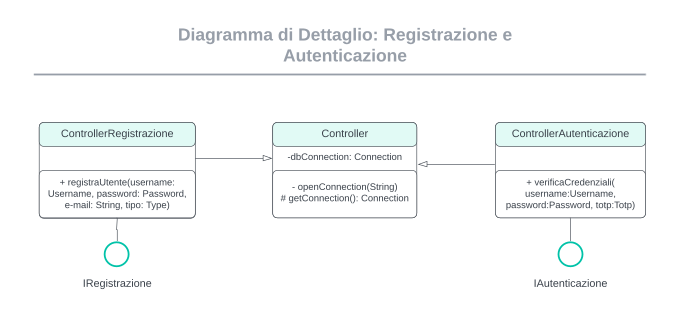
\includegraphics[width=1\textwidth]{assets/img/controllers/accesso.png}\\
\subsubsection{Gestione dell'account personale}
\begin{center}
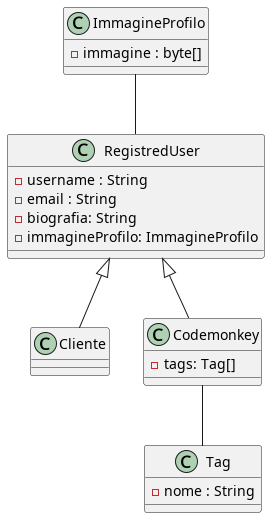
\includegraphics[width=0.35\textwidth]{assets/plantuml/account.png}\\
\end{center}
\subsubsection{Gestione delle Collaborazioni}
\noindent\resizebox{\textwidth}{!}{
    \begin{tikzpicture}
        \fontsize{8}{9.5}\selectfont

        \begin{class}[text width=5cm, fill=green!20, draw=black]{Collaborazione}{0,0}
            \attribute{id : Integer}
            \attribute{titolo : Titolo}
            \attribute{stato: StatoCollaborazione}
            \attribute{descrizioneCollaborazione: DescrizioneCollaborazione}
            \attribute{tags: Tag[]}
            \attribute{valutazione: Valutazione}
            \attribute{codemonkey: Codemonkey}
            \attribute{client: Cliente}
            \attribute{dataProposta: DateTime}
            \attribute{dataAccettazione: DateTime}
            \attribute{dataTerminazione: DateTime}
        \end{class}

        %%%%%%%%%% 

        \begin{class}[text width=5cm, fill=green!20, draw=black, rectangle split parts=2, left=4cm of Collaborazione]{StatoCollaborazione}{0,0}
            \attribute{PROPOSTA}
            \attribute{ACCETTATA}
            \attribute{RIFIUTATA}
            \attribute{INTERROTTA}
            \attribute{TERMINATA}
        \end{class}

        \node [above of=StatoCollaborazione, node distance=1.6cm] (enumeration) {$<<$enumeration$>>$};

        \draw [-{Latex}] (Collaborazione) -- (StatoCollaborazione) node[pos=0.25, above] {1} node[pos=0.75, above] {n};

        %%%%%%%%%%
        
        \begin{class}[text width=5cm, fill=green!20, draw=black, left=4cm of Collaborazione, yshift=4cm]{Valutazione}{0,0}
            \attribute{rating : Float}
            \attribute{commento : String}
            \operation{setRating(Float) : void}
            \operation{setCommento(String) : void}
            \operation{getRating() : Float}
            \operation{getCommento() : String}
        \end{class}

        \draw [-{Latex}] (Collaborazione) -- (Valutazione) node[pos=0.25, above] {1} node[pos=0.75, above] {n};

        %%%%%%%%%% 

        \begin{class}[text width=5cm, fill=green!20, draw=black, right=4cm of Collaborazione, yshift=0cm]{Tag}{0,0}
            \attribute{nome : String}
            \operation{setNome(String) : void}
            \operation{getNome() : String}
        \end{class}

        \draw [-{Latex}] (Collaborazione) -- (Tag) node[pos=0.25, above] {1} node[pos=0.75, above] {n};

        %%%%%%%%%% 

        \begin{class}[text width=5cm, fill=green!20, draw=black, right=4cm of Collaborazione, yshift=3cm]{Titolo}{0,0}
            \attribute{titolo : String}
            \operation{setTitolo(String) : void}
            \operation{getTitolo() : String}
        \end{class}

        \draw [-{Latex}] (Collaborazione) -- (Titolo) node[pos=0.25, above] {1} node[pos=0.75, above] {1};


        %%%%%%%%%% 

        \begin{class}[text width=5cm, fill=green!20, draw=black, right=4cm of Collaborazione, yshift=-3cm]{DescrizioneCollaborazione}{0,0}
            \attribute{descrizioneCollaborazione : String}
            \operation {setDescrizioneCollaborazione(String) : void}
            \operation {getDescrizioneCollaborazione() : String}
        \end{class}

        \draw [-{Latex}] (Collaborazione) -- (DescrizioneCollaborazione) node[pos=0.25, above] {1} node[pos=0.75, above] {1};

        %%%%%%%%%% 


        \begin{class}[text width=8cm, fill=green!20, draw=black, below=7cm of Collaborazione, xshift=-5cm]{Cliente}{0,0}
            \operation{proponiCollaborazione(Codemonkey, Titolo, DescrizioneCollaborazione, Tag[]) : void}
            \operation{modificaCollaborazione(Collaborazione,Codemonkey, Titolo, DescrizioneCollaborazione, Tag[]) : void}
            \operation{terminaCollaborazione(Collaborazione, Valutazione) : void}
        \end{class}

        \draw [-] (Collaborazione) -- (Cliente) node[pos=0.25, right] {1} node[pos=0.75, left] {n};


        \draw [-] (Cliente.west) -- ++(-1,0cm) node[midway, above] {1};
        \draw [-] ([xshift=-1cm]Cliente.west) -- ([xshift=-1cm]Valutazione.west);
        \draw [-{Latex}] ([xshift=-1cm]Valutazione.west) -- (Valutazione.west) node[midway, above] {n};
        
        %%%%%%%%%% 

        \begin{class}[text width=8cm, fill=green!20, draw=black,below=7cm of Collaborazione, xshift=5cm]{Codemonkey}{0,0}
            \operation{accettaCollaborazione(Collaborazione) : void}
            \operation{rifiutaCollaborazione(Collaborazione) : void}
            \operation{interrompiCollaborazione(Collaborazione) : void}
        \end{class}

        \draw [-] (Collaborazione) -- (Codemonkey) node[pos=0.25, above] {1} node[pos=0.75, above] {n};
        
        %%%%%%%%%%%

        % \begin{class}[text width=8cm, fill=green!20, draw=black, below=11cm of Collaborazione, xshift=0cm]{LogCollaborazione}{0,0}
        %     \operation{proponiCollaborazione(Collaborazione) : Log}
        %     \operation{accettaCollaborazione(Collaborazione) : Log}
        %     \operation{rifiutaCollaborazione(Collaborazione) : Log}
        %     \operation{interrompiCollaborazione(Collaborazione) : void}
        %     \operation{terminaCollaborazione(Collaborazione) : Log}
        % \end{class}
        
        % \draw [-{Latex[]}] (Cliente) -- (LogCollaborazione);
        % \draw [-{Latex[]}] (Codemonkey) -- (LogCollaborazione);
        
        \begin{class}[text width=5cm, fill=green!20, draw=black, below=11cm of Collaborazione]{Log}{0,0}
        \end{class}
        \draw [-{Latex[]}] (Cliente) -- (Log);
        \draw [-{Latex[]}] (Codemonkey) -- (Log);



    \end{tikzpicture}
}
\subsubsection{Gestione dei Tag}
\noindent\resizebox{\textwidth}{!}{
    \begin{tikzpicture}
        \fontsize{8}{9.5}\selectfont

        \begin{class}[text width=5cm, fill=green!20, draw=black]{Tag}{0,0}
            \attribute{nome: String}
            \attribute{stato: StatoTag}
            \attribute{dataProposta: DateTime}
        \end{class}

        %%%%%%%%%% 

        \begin{class}[text width=5cm, fill=green!20, draw=black, rectangle split parts=2, left=4cm of Tag]{StatoTag}{0,0}
            \attribute{IN\_ATTESA}
            \attribute{APPROVATO}
            \attribute{RIFIUTATO}
        \end{class}

        \node [above of=StatoTag, node distance=1.6cm] (enumeration) {$<<$enumeration$>>$};

        \draw [{Diamond}-] (Tag) -- (StatoTag) node[pos=0.25, above] {1} node[pos=0.75, above] {n};

        %%%%%%%%%%
        
        \begin{class}[text width=5cm, fill=green!20, draw=black, below=4cm of Tag, xshift=-4cm]{Codemonkey}{0,0}
            \operation{proponiTag(String) : void}
        \end{class}
        
        \draw [-{Latex[open]}] (Codemonkey) -- (Tag);

        %%%%%%%%%%
        
        \begin{class}[text width=5cm, fill=green!20, draw=black, below=4cm of Tag, xshift=4cm]{Admin}{0,0}
            \operation{accettaTag(Tag) : void}
            \operation{rifiutaTag(Tag) : void}
        \end{class}
        
        \draw [-{Latex[open]}] (Admin) -- (Tag);

        %%%%%%%%%%%

        \begin{class}[text width=5cm, fill=green!20, draw=black, below=6cm of Tag]{Action}{0,0}
        \end{class}
        \draw [-{Latex[]}] (Codemonkey) -- (Action);
        \draw [-{Latex[]}] (Admin) -- (Action);

    \end{tikzpicture}
}
\subsubsection{Gestione delle Segnalazioni}
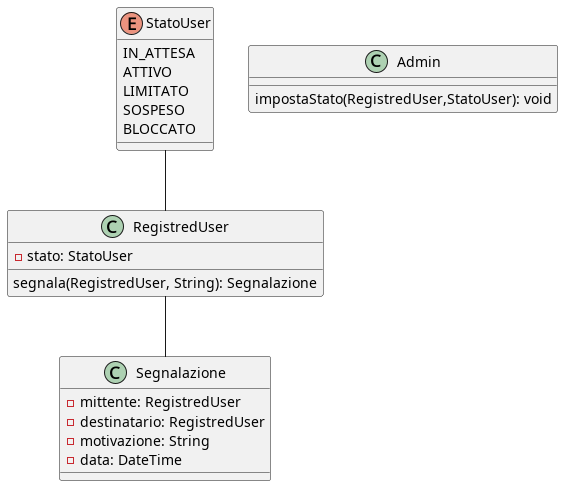
\includegraphics[width=1\textwidth]{assets/plantuml/report.png}\\
\subsubsection{Gestione dei Log}
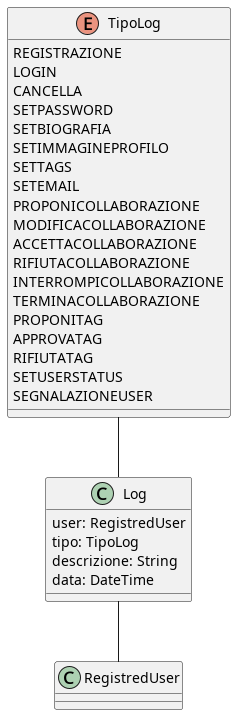
\includegraphics[width=0.25\textwidth]{assets/plantuml/log.png}\\


\pagebreak
\begin{center}

    Il progetto e lo sviluppo del sistema sono assegnati a diversi team come indicato nella tabella sottostante:
    \\\phantom{M}

    \begin{tabularx}{\textwidth}{|X|X|}
        \hline \textbf{Team} & \textbf{Persone assegnate}
        \n Team Prgettazione & Alessandro, Stefano, Valerio
        \n Team sviluppo     & Alessandro, Stefano, Valerio
        \n Team DB           & Alessandro, Stefano, Valerio
        \n Team sicurezza    & Alessandro, Stefano, Valerio
        \n Team grafico      & Alessandro, Stefano, Valerio
        \n
    \end{tabularx}

    \phantom{M}

    \begin{tabularx}{\textwidth}{|X|X|X|}

        \hline \textbf{Package} & \textbf{Progetto} & \textbf{Sviluppo}
        \n        Interfaccia Registrazione      &  Team Progettazione + Team Grafico     &   Team Sicurezza + Team Grafico
        \n   Interfaccia Utente       & Team Progettazione + Team Grafico   & Team Sviluppo + Team Grafico
        \n    Interfaccia Cliente    &  Team Progettazione + Team Grafico  & Team Sviluppo + Team Grafico
        \n      Interfaccia CodeMonkey    &  Team Progettazione + Team Grafico  & Team Sviluppo + Team Grafico
        \n     Interfaccia Utente Registrato      &  Team Progettazione + Team Grafico  &   Team Sviluppo + Team Grafico 
        \n      Interfaccia Autenticazione     &  Team Progettazione + Team Grafico  &  Team Sicurezza + Team Grafico
        \n      Interfaccia Amministratore     &  Team Progettazione + Team Grafico  & Team Sviluppo + Team Grafico
        \n      Registrazione     &  Team Sicurezza   & Team Sviluppo Sicurezza 
        \n        Autenticazione   &  Team Sicurezza  & Team Sviluppo Sicurezza
        \n       Log      &  Team Sicurezza  & Team Sviluppo Sicurezza
        \n       Homepage    &   Team progettazione + Team Grafico  & Team Sviluppo + Team Grafico
        
        \n       Gestione Collaborazioni Cliente    &  Team Progettazione  & Team Sviluppo 
        \n
    \end{tabularx}

    \begin{tabularx}{\textwidth}{|X|X|X|}

        \hline \textbf{Package} & \textbf{Progetto} & \textbf{Sviluppo}
        \n       Gestione Collaborazioni CodeMonkey    &  Team Progettazione  & Team Sviluppo
        \n       Gestione Collaborazioni    &  Team Progettazione + Team DB  & Team Sviluppo + Team DB
        \n       Gestione Account Utente    & Team Progettazione + Team DB   & Team Sviluppo + Team DB
        \n         Amministrazione  &  Team Progettazione + Team DB & Team Sviluppo + Team DB
        \n
    \end{tabularx}
\end{center}
Nel futuro verrá costruita una chat interna alla piattaforma per permettere un dialogo fra Codemonkey e Cliente, eliminando il bisogno di utlilizzare strumenti esterni.


\end{document}
